% Master's-defense slides for the thesis.
% Build:  latexmk -pdf slides.tex          (pdflatex; robust, no font install needed)
% Nicer:  latexmk -pdflua slides.tex       (lualatex + Fira Sans, the full Metropolis look)
%
% Structure mirrors the thesis's research-question arc:
%   opening (thesis-in-one-breath) -> problem+RQs -> RQ1 characterize ->
%   RQ2 forecast -> RQ3 platform -> RQ4 closed loop -> validation & scope ->
%   contributions.
\documentclass[11pt,aspectratio=169]{beamer}
\usetheme{metropolis}
\metroset{block=fill,sectionpage=progressbar,numbering=fraction}

\usepackage[T1]{fontenc}
\usepackage[utf8]{inputenc}
\usepackage[main=english]{babel}
\usepackage{amsmath,amssymb}
\usepackage{siunitx}
\usepackage{booktabs}
\usepackage{graphicx}
\graphicspath{{../figuras/}}
\usepackage{tikz}
\usetikzlibrary{positioning,arrows.meta,calc}
\usepackage{colortbl}
\newcommand{\cmark}{\textcolor{teal!65!black}{\checkmark}}

\title{Predictive Per-Pool Provisioning for\\ Modality-Disaggregated Multimodal Model Serving}
\author{Giovanni Oliveira}
\institute{%
  \scriptsize Advisor: Prof.\ Dr.\ Fabio Kon \quad Co-advisor: Prof.\ Dr.\ Em\'ilio Francesquini\\[0.2ex]
  Programa de P\'os-Gradua\c{c}\~ao em Ci\^encia da Computa\c{c}\~ao\\
  Instituto de Matem\'atica e Estat\'istica --- Universidade de S\~ao Paulo, S\~ao Paulo, Brasil}
\date{\today}

\begin{document}

\maketitle

% ------------------------------------------------------------------
\begin{frame}{The thesis in one breath}
  \begin{enumerate}
    \item Multimodal serving splits into separately-provisioned \textbf{vision} and
          \textbf{language} GPU pools --- but autoscaling watches \emph{one} reactive
          signal (request rate / utilization).
    \item On the first public multimodal production trace, the vision pool's demand is
          \alert{nearly decoupled from request rate} ($R^2{=}0.12$) --- yet \alert{persistent
          enough to forecast} (Hurst $0.93$).
    \item Zero-shot time-series foundation models turn each pool's \emph{own} signal
          into a worker schedule, on a silicon-calibrated two-pool platform.
    \item Result: the tail-latency SLA \textbf{holds through every in-span burst} that
          defeats a same-signal reactive baseline (trailing point rate, no p90 headroom) ---
          at \alert{$0.62\times$} the deployable static encoder fleet's GPU-time.
  \end{enumerate}
\end{frame}

\begin{frame}{Outline}
  \tableofcontents
\end{frame}

% ------------------------------------------------------------------
\section{Problem and research questions}

\begin{frame}{Multimodal serving disaggregates by modality}
  A multimodal request splits across two separately-provisioned GPU pools:
  \begin{itemize}
    \item \textbf{Vision / encoder pool} --- images $\to$ embedding tokens (a ViT).
    \item \textbf{Language pool} --- prefill $+$ decode (the LLM).
  \end{itemize}
  \vfill
  Modern stacks (NVIDIA Dynamo, \ldots) size each pool on its own --- but the prevailing
  practice is \textbf{reactive} scaling on request rate or GPU utilization, assuming
  those signals carry \emph{every} pool's demand.
  \vfill
  \alert{Does the request-rate signal actually capture the \emph{vision} pool's demand?
  And if not, what should size that pool?}
\end{frame}

\begin{frame}{Research questions (= the chapter arc)}
  \begin{description}[<+->]
    \item[RQ1 --- Characterize.] Is the vision pool's demand \textbf{decoupled} from the
      signals reactive autoscalers watch --- and what temporal structure does it have?
    \item[RQ2 --- Forecast.] Is that demand \textbf{forecastable at provisioning
      horizons}, and by what kind of model?
    \item[RQ3 --- Model.] Does a \textbf{silicon-calibrated two-pool platform} reproduce
      the decoupling \emph{mechanically} --- where does each pool actually break?
    \item[RQ4 --- Close the loop.] Do \textbf{forecast-driven per-pool schedules} hold
      the tail SLA --- and at what cost against reactive and static fleets?
  \end{description}
  \onslide<4->{%
  \vspace{0.6ex}\centering\resizebox{0.9\linewidth}{!}{%
  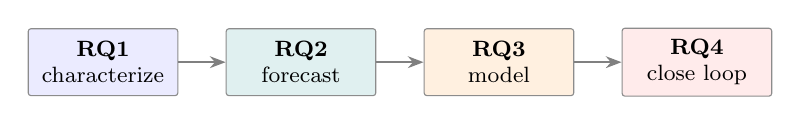
\begin{tikzpicture}[font=\footnotesize,
    chev/.style={draw=black!45, rounded corners=1pt, inner sep=4pt, align=center,
                 minimum height=0.85cm, minimum width=1.9cm},
    arr/.style={-{Stealth[length=2mm]}, thick, black!50}]
  \node[chev, fill=blue!8] (a) {\textbf{RQ1}\\characterize};
  \node[chev, fill=teal!12, right=6mm of a] (b) {\textbf{RQ2}\\forecast};
  \node[chev, fill=orange!12, right=6mm of b] (c) {\textbf{RQ3}\\model};
  \node[chev, fill=red!8, right=6mm of c] (d) {\textbf{RQ4}\\close loop};
  \draw[arr] (a)--(b); \draw[arr] (b)--(c); \draw[arr] (c)--(d);
  \end{tikzpicture}}}
\end{frame}

\begin{frame}{Positioning: no prior system closes all four gaps}
  \centering
  \footnotesize
  \setlength{\tabcolsep}{5pt}\renewcommand{\arraystretch}{1.0}
  \begin{tabular}{@{}>{\raggedright\arraybackslash}p{3.7cm}ccccc@{}}
    \toprule
      & Modality & Per-pool & Forecast & Calibrated & Real-cluster \\
    Work & disagg. & signals & scaling & simulation & GPU eval. \\
    \midrule
    ModServe                 & \cmark & \cmark & ---    & ---    & \cmark \\
    EPD / HydraInfer         & \cmark & ---    & ---    & ---    & \cmark \\
    ElasticMM                & \cmark & $\sim$ & $\sim$ & ---    & \cmark \\
    SageServe / WarmServe    & ---    & ---    & \cmark & ---    & \cmark \\
    TokenScale / HeteroScale & ---    & $\sim$ & $\sim$ & ---    & \cmark \\
    Dynamo (planner)         & $\sim$ & ---    & $\sim$ & $\sim$ & \cmark \\
    Vidur / LLMServingSim 2.0& ---    & ---    & ---    & $\sim$ & $\sim$ \\
    \midrule
    \rowcolor{blue!8}\textbf{This thesis} & \cmark & \cmark & \cmark & \cmark & $\sim$ \\
    \bottomrule
  \end{tabular}
  \vspace{0.7ex}\par
  {\scriptsize \cmark~full \quad $\sim$~partial/heuristic \quad ---~none \qquad
  The only row combining \textbf{per-pool forecast-driven scaling} with a
  \textbf{calibrated cost model}; real-cluster eval.\ is $\sim$ (mocked engines).}
\end{frame}

% ------------------------------------------------------------------
\section{RQ1 --- A decoupled, bursty, persistent vision signal}

\begin{frame}{Dataset characterization: the trace at a glance}
  \begin{columns}[T]
    \begin{column}{0.42\textwidth}
      \footnotesize
      \begin{tabular}{@{}ll@{}}
        \multicolumn{2}{@{}l}{\textbf{Azure LMM trace} {\scriptsize(w/ ModServe, 2025)}}\\
        \midrule
        Scale     & 1M requests, 7 days \\
        Eval span & 5.6 days (post-warmup) \\
        Signals   & req/s, img/s, tok/s \\
        \addlinespace
        \multicolumn{2}{@{}l}{\textbf{The vision signal is\ldots}}\\
        \midrule
        decoupled   & $R^2{=}0.12$ vs.\ req rate \\
        heavy-tailed& 2.7\% req $\to$ 81.2\% imgs \\
        bursty      & Fano $1.8\to938$ (1\,s--1\,h) \\
        disjoint    & Jaccard 0.02 at the extremes \\
        \textbf{persistent} & \textbf{Hurst 0.93}, long half-life \\
        \bottomrule
      \end{tabular}
    \end{column}
    \begin{column}{0.58\textwidth}
      \centering\includegraphics[width=\linewidth]{fig/eda_c_seven_day_signals}
    \end{column}
  \end{columns}
\end{frame}

\begin{frame}{The decoupling: request rate cannot see vision demand}
  \begin{columns}[T]
    \begin{column}{0.52\textwidth}
      \begin{itemize}
        \item Image arrivals vs.\ request rate: $R^2 = 0.12$ --- a forced
              through-origin fit ($15.1$ img/req) explains almost nothing.
        \item A small \textbf{``frames class''} ($k^2$ image grids: 2.7\% of requests)
              carries \textbf{81.2\% of image volume}.
        \item Extremes are disjoint (Jaccard 0.02): the busiest \emph{request} minutes
              are not the busiest \emph{image} minutes.
        \item[$\Rightarrow$] request-rate and window-mean-utilization monitors
              \textbf{cannot see} the vision pool's demand.
      \end{itemize}
    \end{column}
    \begin{column}{0.48\textwidth}
      \centering\includegraphics[width=\linewidth,height=0.72\textheight,keepaspectratio]{fig/eda_d_img_vs_req_scatter}
    \end{column}
  \end{columns}
\end{frame}

\begin{frame}{\ldots but that demand is the most \emph{persistent}}
  \begin{itemize}
    \item Bursty yet strongly \textbf{persistent} (long-range dependence, Hurst
          ${\approx}0.93$); burst \emph{onsets} unfold over minutes --- the horizon a
          provisioner needs. The decoupling that blinds reactive autoscaling is paired with
          the persistence that enables \emph{anticipation}.
  \end{itemize}
  \centering\includegraphics[width=0.86\linewidth,height=0.54\textheight,keepaspectratio]{fig/eda_i_burst_onsets}
\end{frame}

% ------------------------------------------------------------------
\section{RQ2 --- Forecastable at provisioning horizons}

\begin{frame}{Zero-shot foundation models forecast the pool signals}
  \begin{itemize}
    \item Chronos-2, Toto-2, TimesFM --- \textbf{zero-shot}, rolling-origin on every
          (signal, resolution) cell: near the per-cell optimum \textbf{everywhere} (light),
          while baselines darken as bins shrink. Covariates \textbf{don't help} the image
          signal (the $R^2{=}0.12$ decoupling).
  \end{itemize}
  \centering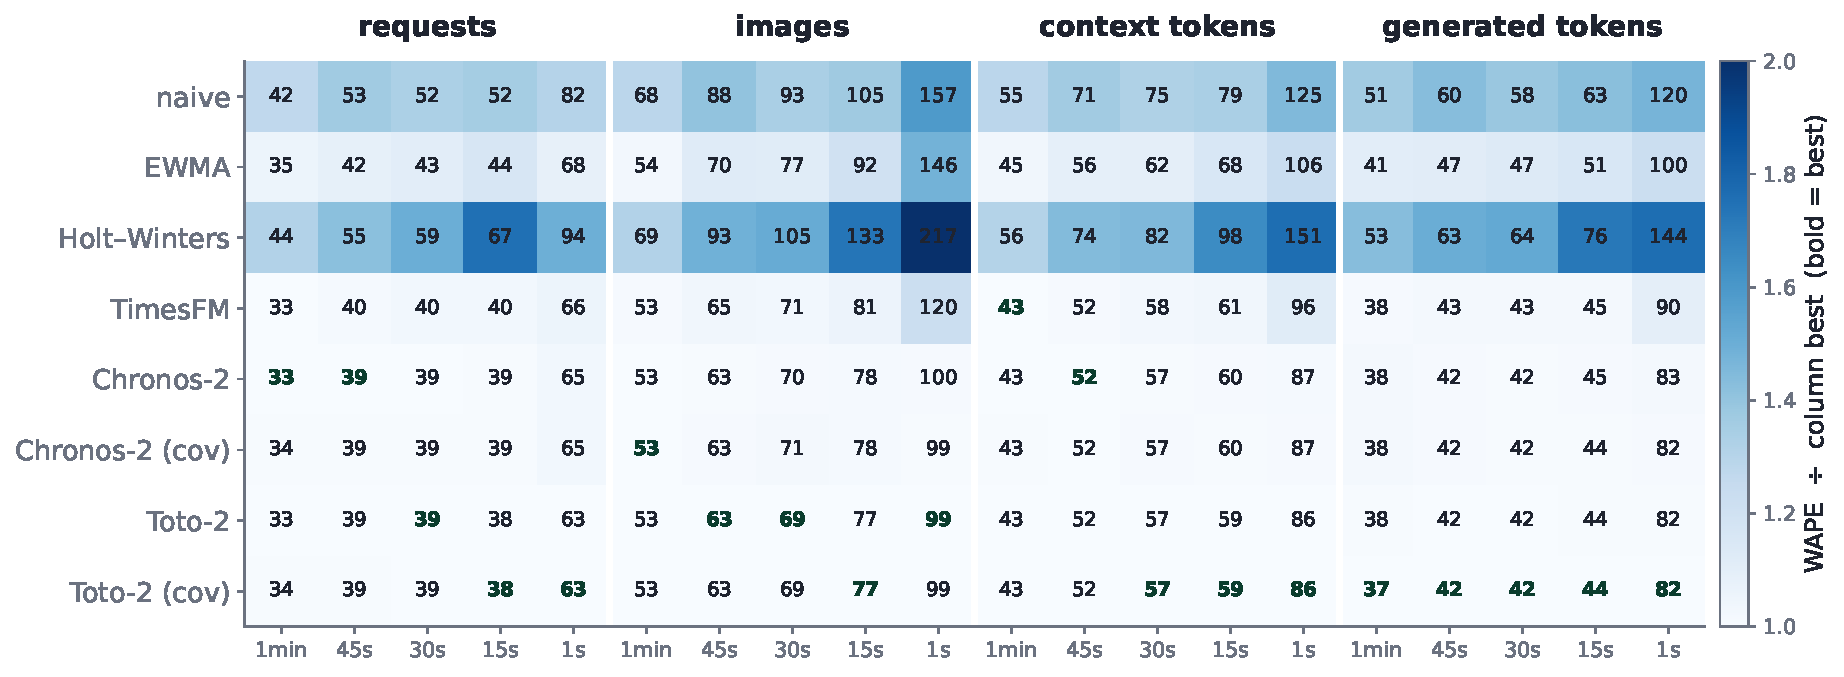
\includegraphics[width=0.99\linewidth,height=0.54\textheight,keepaspectratio]{fig/pred_heatmap_slide}
\end{frame}

\begin{frame}{What makes a forecast provisioning-grade}
  \begin{itemize}
    \item Skill holds across the \textbf{12-step horizon} (figure: 1-min resolution,
          $h{=}1$--$12$\,min); the closed-loop controller reads a separate 15-s archive
          ($\to 15$--$165$\,s issued lead). The calibrated \textbf{p90 band} (coverage
          0.88--0.90) turns a point forecast into provisionable \emph{headroom} ---
          \textbf{which} TSFM matters less than \textbf{how} its band is consumed.
  \end{itemize}
  \centering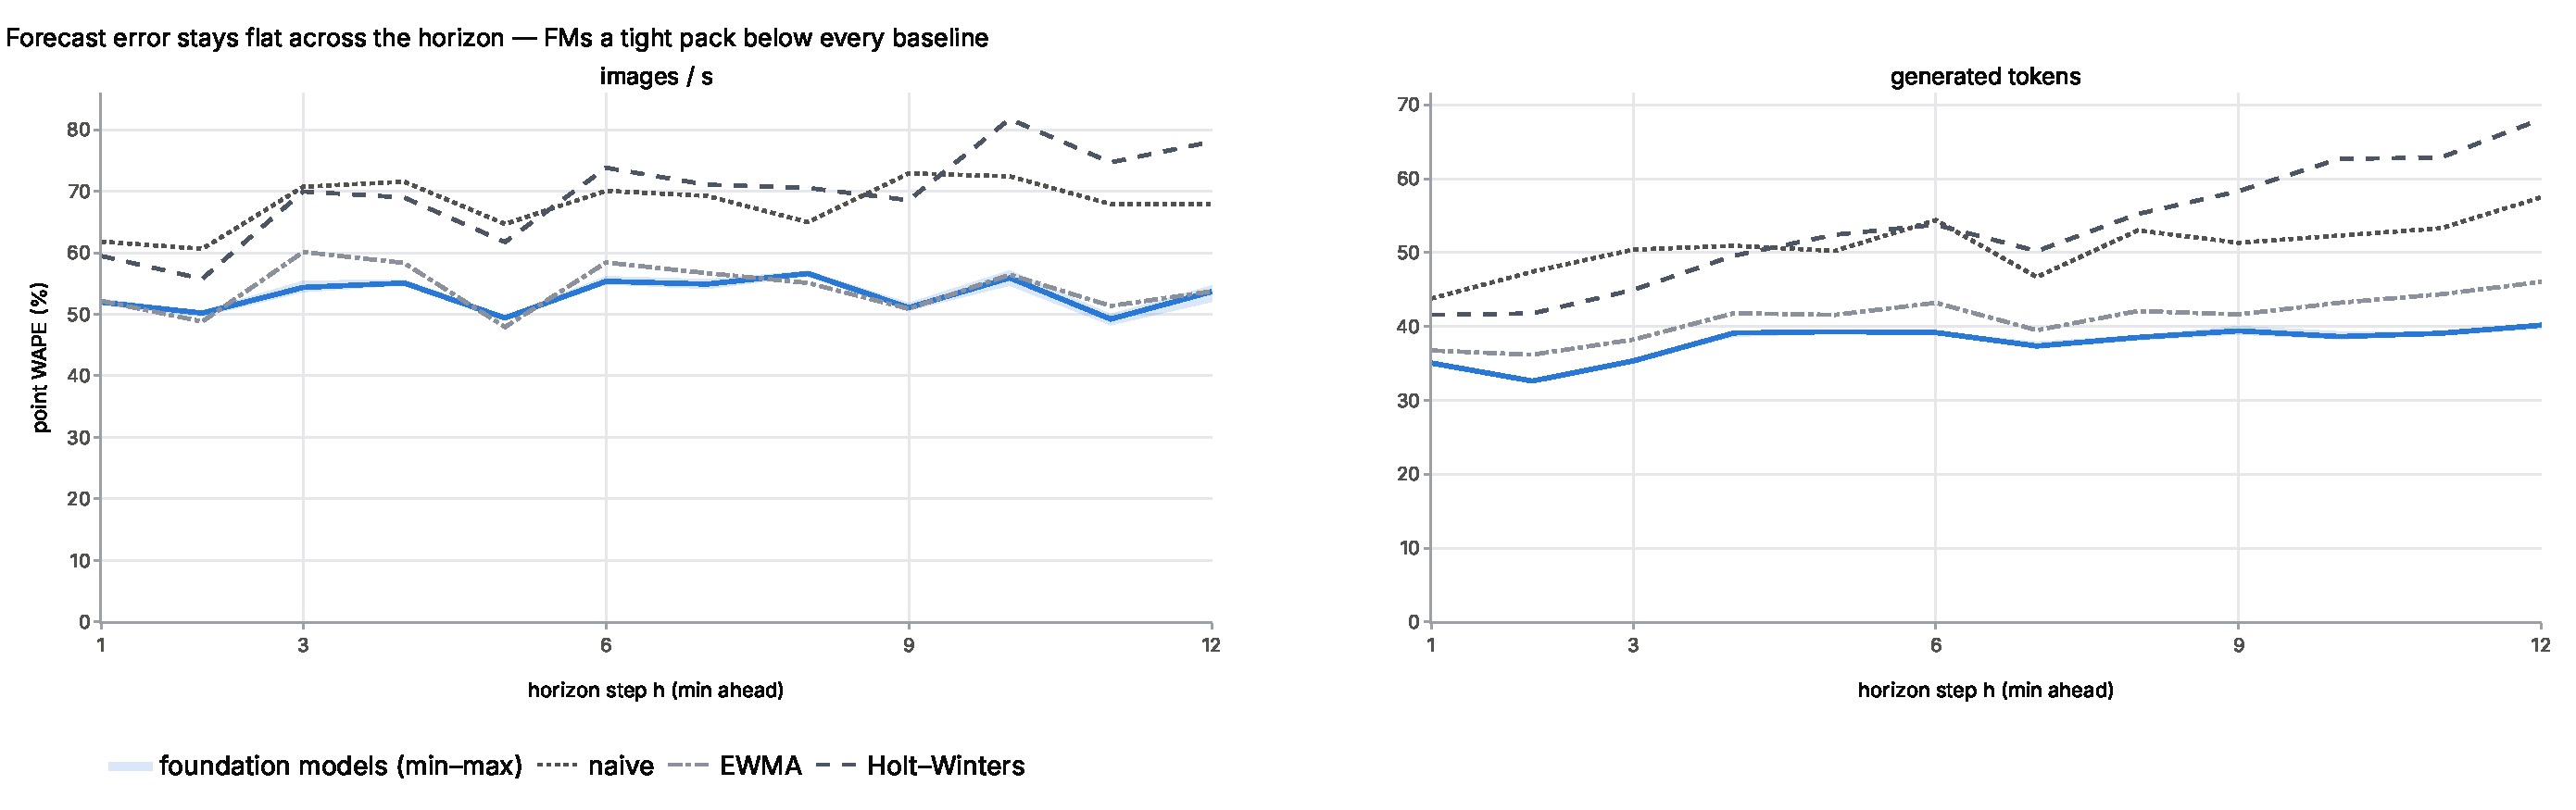
\includegraphics[width=0.92\linewidth,height=0.54\textheight,keepaspectratio]{fig/pred_horizon_slide}
\end{frame}

% ------------------------------------------------------------------
\section{RQ3 --- A silicon-calibrated two-pool platform}

\begin{frame}{System architecture: the two-pool simulator}
  \centering
  \resizebox{0.97\linewidth}{!}{%
  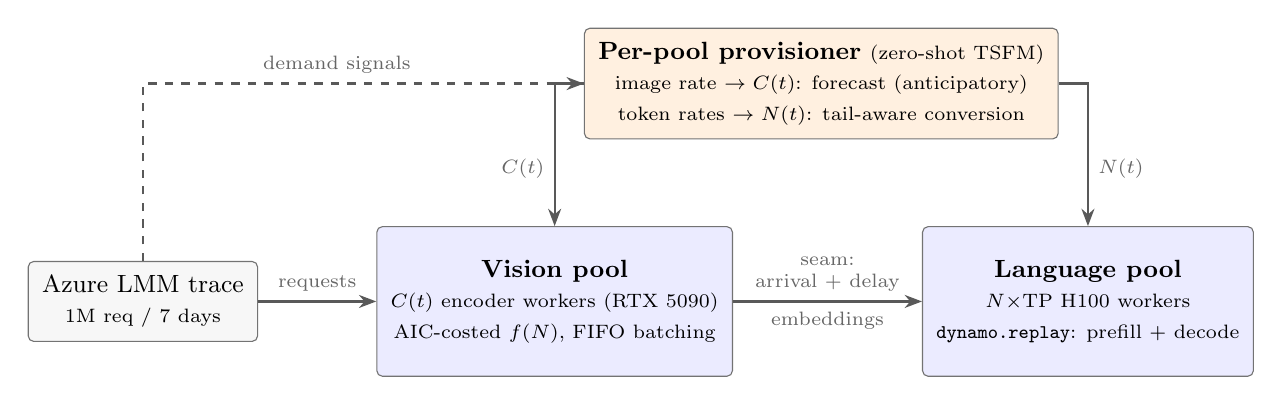
\begin{tikzpicture}[
    font=\small,
    box/.style={draw=black!55, rounded corners=2pt, align=center, inner sep=5pt, fill=black!3},
    pool/.style={box, fill=blue!8, minimum height=1.9cm},
    ctrl/.style={box, fill=orange!12},
    arr/.style={-{Stealth[length=2.2mm]}, thick, black!65},
    lbl/.style={font=\scriptsize, black!60, align=center},
  ]
  \node[box] (trace) {Azure LMM trace\\\scriptsize 1M req / 7 days};
  \node[pool, right=1.5cm of trace] (vis) {\textbf{Vision pool}\\
    \scriptsize $C(t)$ encoder workers (RTX~5090)\\\scriptsize AIC-costed $f(N)$, FIFO batching};
  \node[pool, right=2.4cm of vis] (llm) {\textbf{Language pool}\\
    \scriptsize $N{\times}$TP H100 workers\\\scriptsize \texttt{dynamo.replay}: prefill + decode};
  \node[ctrl, above=1.1cm of $(vis.north)!0.5!(llm.north)$] (fc)
    {\textbf{Per-pool provisioner} {\scriptsize(zero-shot TSFM)}\\
    \scriptsize image rate $\to C(t)$: forecast (anticipatory)\\
    \scriptsize token rates $\to N(t)$: tail-aware conversion};
  \draw[arr] (trace) -- node[lbl, above] {requests} (vis);
  \draw[arr] (vis) -- node[lbl, above] {seam:\\arrival $+$ delay} node[lbl, below] {embeddings} (llm);
  \draw[arr] (fc.west) -| node[lbl, left, pos=0.8] {$C(t)$} (vis.north);
  \draw[arr] (fc.east) -| node[lbl, right, pos=0.8] {$N(t)$} (llm.north);
  \draw[arr, dashed] (trace.north) |- node[lbl, above, pos=0.72] {demand signals} (fc.west);
  \end{tikzpicture}}
  \vfill
  {\footnotesize An AIC-costed encoder pool composed with Dynamo's H100 language pool through a
  timestamp-shift seam; the provisioner sizes each pool from its \emph{own} demand signal.}
\end{frame}

\begin{frame}{Encoder costs collected --- and validated --- on real silicon}
  \begin{itemize}
    \item Cost model \textbf{collected on RTX~5090} (contributed upstream, draft PR \#1312) and
          \textbf{validated} against vLLM's own vision tower over a dense 69-point sweep
          ($N{=}1$--$512$); the $N{\le}64$ serving regime agrees within \textbf{12.8\%}.
  \end{itemize}
  \centering\includegraphics[width=0.98\linewidth,height=0.58\textheight,keepaspectratio]{fig/aic_fn_engines}
\end{frame}

\begin{frame}{The mechanics of decoupling: knees an order of magnitude apart}
  \begin{itemize}
    \item On steady traffic the knees sit \textbf{${>}10\times$ apart} (an order of magnitude).
          During the largest burst \textbf{both pools fail}, for structurally different reasons:
          language, a shape-fixable prefill floor (removed by TP2); vision, \textbf{episodic
          encoder queueing at 29\% \emph{mean} utilization}, which yields only to capacity.
          RQ1's decoupling, reproduced \emph{mechanically}.
  \end{itemize}
  \centering\includegraphics[width=0.9\linewidth,height=0.44\textheight,keepaspectratio]{fig/sim_knees}
\end{frame}

% ------------------------------------------------------------------
\section{RQ4 --- Forecast-driven provisioning closes the loop}

\begin{frame}{Per-pool mechanism: each pool provisioned from its own signal}
  \centering
  \resizebox{0.98\linewidth}{!}{%
  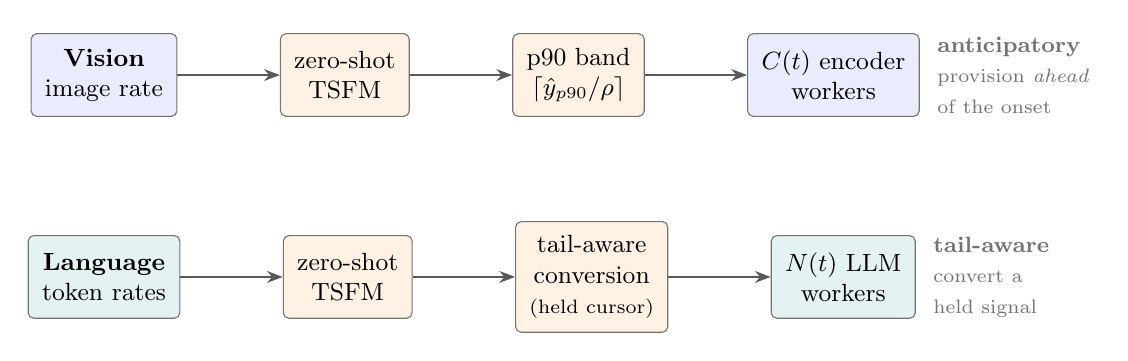
\begin{tikzpicture}[
    font=\small, node distance=10mm and 13mm,
    b/.style={draw=black!55, rounded corners=2pt, align=center, inner sep=5pt, minimum height=1.05cm},
    enc/.style={b, fill=blue!8}, lan/.style={b, fill=teal!10}, op/.style={b, fill=orange!10},
    arr/.style={-{Stealth[length=2mm]}, thick, black!65},
    lbl/.style={font=\scriptsize\itshape, black!55},
  ]
  % encoder (vision) row
  \node[enc] (e1) {\textbf{Vision}\\image rate};
  \node[op, right=of e1] (e2) {zero-shot\\TSFM};
  \node[op, right=of e2] (e3) {p90 band\\$\lceil \hat{y}_{p90}/\rho\rceil$};
  \node[enc, right=of e3] (e4) {$C(t)$ encoder\\workers};
  \draw[arr] (e1)--(e2); \draw[arr] (e2)--(e3); \draw[arr] (e3)--(e4);
  \node[black!55, right=1mm of e4, align=left] {\footnotesize\textbf{anticipatory}\\\scriptsize provision \emph{ahead}\\\scriptsize of the onset};
  % language row
  \node[lan, below=1.5cm of e1] (l1) {\textbf{Language}\\token rates};
  \node[op, right=of l1] (l2) {zero-shot\\TSFM};
  \node[op, right=of l2] (l3) {tail-aware\\conversion\\{\scriptsize(held cursor)}};
  \node[lan, right=of l3] (l4) {$N(t)$ LLM\\workers};
  \draw[arr] (l1)--(l2); \draw[arr] (l2)--(l3); \draw[arr] (l3)--(l4);
  \node[black!55, right=1mm of l4, align=left] {\footnotesize\textbf{tail-aware}\\\scriptsize convert a\\\scriptsize held signal};
  \end{tikzpicture}}
  \vfill
  {\footnotesize One zero-shot forecaster, two actuations --- the encoder provisions \emph{ahead} of
  the onset; the language pool \emph{converts} the held signal into tail-aware headroom.
  Quantile (p90) and cold-start lead $L$ are the shared dials.}
\end{frame}

\begin{frame}{Forecast holds the SLA where reactive breaks}
  \begin{itemize}
    \item The p90 forecast policy meets the SLA in \textbf{all 60 issue-time cells}
          (window $\times$ model $\times$ lead), burst p99 pinned at the \SI{588}{\milli\second}
          zero-queueing floor --- while a \textbf{same-signal reactive baseline} (trailing point
          rate, no p90 headroom) loses burst3 at every lead and burst4/5 beyond \SI{45}{\second}.
  \end{itemize}
  \centering\includegraphics[width=0.88\linewidth,height=0.54\textheight,keepaspectratio]{fig/sim_burst_queue}
\end{frame}

\begin{frame}{What makes it work: the ablation ledger}
  \begin{columns}[T]
    \begin{column}{0.6\textwidth}
      \begin{description}
        \item[Quantile is decisive.] p90: 60/60 cells. p50: 23--24/60 --- the median sizes
          to the mean and fails \emph{even the calm day}.
        \item[Lead-invariance.] \emph{Burst} p99 unchanged (pinned \SI{588}{\milli\second}),
          $L{=}15$ to \SI{165}{\second}; the reactive twin degrades monotonically with lead
          --- the signature of anticipation.
        \item[Model is second-order \emph{for the verdict}.] All three TSFMs pass all cells;
          but language-pool \emph{cost} varies 0.96$\times$--1.19$\times$ by model.
      \end{description}
    \end{column}
    \begin{column}{0.4\textwidth}
      \centering
      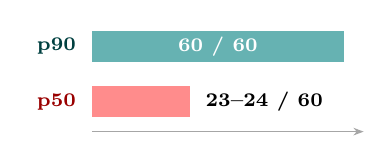
\begin{tikzpicture}[font=\scriptsize]
        \fill[teal!60] (0,0.7) rectangle (3.2,1.1);
        \node[white] at (1.6,0.9) {\textbf{60 / 60}};
        \node[left,teal!50!black] at (-0.08,0.9) {\textbf{p90}};
        \fill[red!45] (0,0) rectangle (1.25,0.4);
        \node[right] at (1.32,0.2) {\textbf{23--24 / 60}};
        \node[left,red!60!black] at (-0.08,0.2) {\textbf{p50}};
        \draw[black!35,-{Stealth[length=1.3mm]}] (0,-0.18)--(3.45,-0.18);
      \end{tikzpicture}
      \\[0.5ex]{\scriptsize issue-time cells passed ($\rho{=}15$)}
    \end{column}
  \end{columns}
\end{frame}

\begin{frame}{Headline economics}
  \begin{block}{Week-scale cost, SLA held}
    Forecast-driven per-pool provisioning serves the week-scale span (5.6 evaluated days) at
    \alert{\textbf{0.62$\times$}} the deployable static \emph{encoder} fleet's GPU-time
    (language pool $\approx$ break-even: $0.96\times$ with Chronos, up to $1.19\times$ with
    other TSFMs).
  \end{block}
  \begin{columns}[T]
    \begin{column}{0.45\textwidth}
      \begin{itemize}
        \item The $\rho$ frontier: $\rho{=}15$ \emph{conservative} headline; $\rho{=}20$
              cheapest clean; $\rho{=}25$ loses burst5.
        \item Survives repricing the encoder at the \textbf{measured} vLLM cost: week-scale
              p99 moves only 589$\to$\SI{606}{\milli\second}, non-divergent, cost unchanged.
      \end{itemize}
    \end{column}
    \begin{column}{0.55\textwidth}
      \centering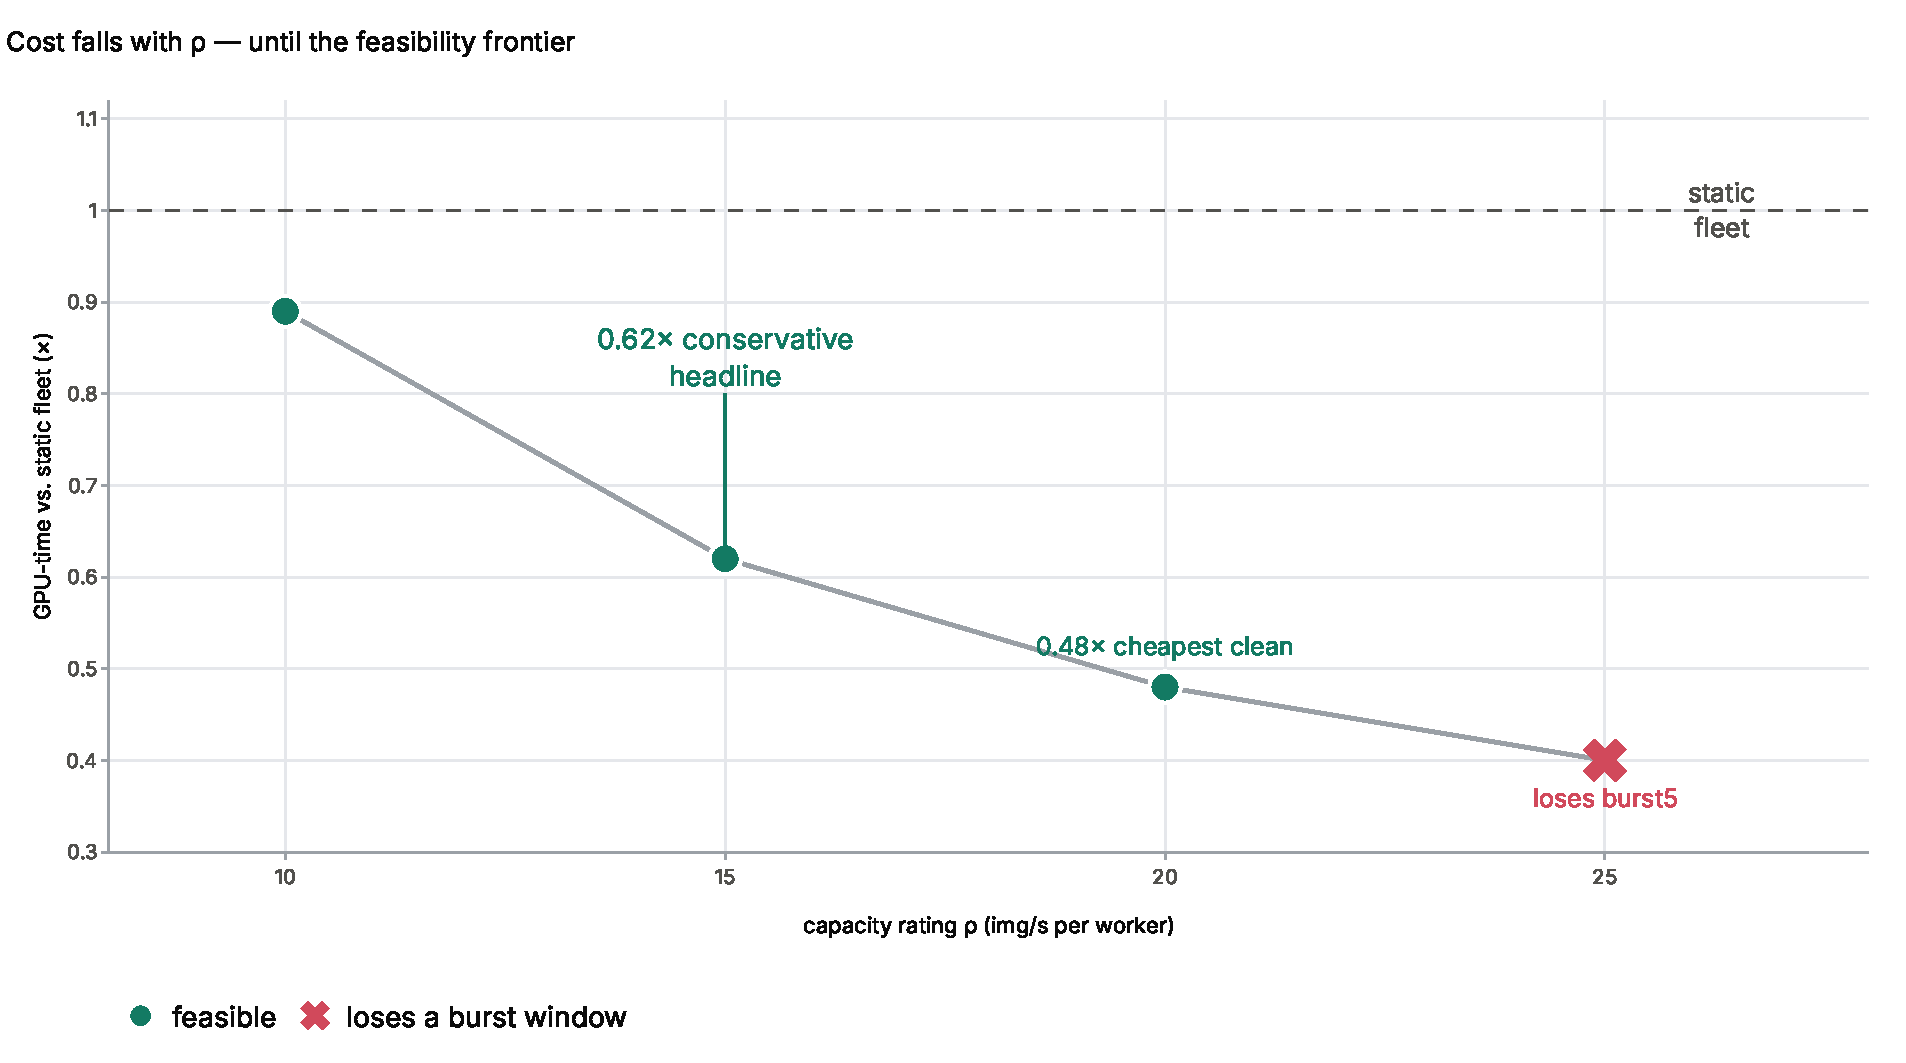
\includegraphics[width=\linewidth,height=0.52\textheight,keepaspectratio]{fig/cost_frontier}
    \end{column}
  \end{columns}
\end{frame}

% ------------------------------------------------------------------
\section{Validation and scope}

\begin{frame}{Three evidence layers behind the claims}
  \begin{enumerate}
    \item \textbf{Statistical honesty} --- rolling-origin, zero-shot forecasts; schedules
          actuated at \emph{issue time} (no look-ahead); no constant tuned on the
          evaluation span; whole frontiers reported ($\rho{=}15$ chosen \emph{ex post} as the
          conservative operating point, not tuned to flatter).
    \item \textbf{Silicon anchoring} --- encoder cost model validated against vLLM's own
          vision tower (within 12.8\% across the serving regime); the week economics
          replayed under the measured cost curve (0.62$\times$ unchanged).
    \item \textbf{Live control plane} --- on the fastest-onset burst (burst3), the
          p90-vs-reactive verdict pair reproduces through Dynamo's \emph{real} control
          plane (language pool, one live run per policy; planner, etcd/NATS, KV router;
          mocked engines), client-observed TTFT within 1.1--6.8\% of the offline replay.
  \end{enumerate}
\end{frame}

\begin{frame}{Scope and future work}
  \begin{columns}[T]
    \begin{column}{0.5\textwidth}
      \textbf{Scope}
      \begin{itemize}
        \item One Azure trace, 5.6-day evaluation span; one model family.
        \item Live loop: real control plane, \textbf{mocked engines}.
        \item Encoder measured as a standalone forward (not the full serving path).
      \end{itemize}
    \end{column}
    \begin{column}{0.5\textwidth}
      \textbf{Future work}
      \begin{itemize}
        \item A live encoder worker over the full serving path.
        \item Multi-node disaggregated deployment (Grove).
        \item Other engines/backends (SGLang, TRT-LLM).
        \item Beyond one trace: other workloads, models, datacenters.
      \end{itemize}
    \end{column}
  \end{columns}
\end{frame}

% ------------------------------------------------------------------
\section{Contributions}

\begin{frame}{Contributions}
  \begin{enumerate}
    \item \textbf{To our knowledge}, first to \textbf{quantify} the modality decoupling ModServe
          noted only \emph{qualitatively} ($R^2{=}0.12$, frames class, persistence) --- and to frame
          the pool signals as \textbf{forecasting targets}, not reactive load. \hfill{\scriptsize RQ1}
    \item \textbf{Per-pool forecastability}: zero-shot time-series foundation models as
          provisioning signals, with calibrated quantile headroom. \hfill{\scriptsize RQ2}
    \item A \textbf{silicon-calibrated two-pool platform} (RTX~5090 encoder, contributed upstream
          as draft PR \#1312; Dynamo H100 language) reproducing the decoupling mechanically. \hfill{\scriptsize RQ3}
    \item \textbf{Forecast-driven per-pool provisioning}: the tail SLA held through every
          in-span burst at $0.62\times$ static \emph{encoder} GPU-time --- issue-time honest,
          cost silicon-anchored --- with the burst verdict further reproduced through a live
          control plane (language pool, mocked engines). \hfill{\scriptsize RQ4}
  \end{enumerate}
\end{frame}

\begin{frame}[standout]
  Thank you.\\[1.5ex]
  \normalsize Questions?
\end{frame}

\end{document}
